\chapter{Realizace}\label{realizace}

Pro realizaci aplikace byl použit herní engine \emph{Unity}.
\emph{Unity} je multi-platformní herní engine napsaný v~C a C++, určený
k~vývoji her pro PC, konzole a mobilní zařízení. Je to v~současnosti
jeden z~nejvhodnějších a nejpopulárnějších nástrojů na vývoj her pro
virtuální realitu. \autocite{unitypopularity}

Ač jde o~nástroj pro tvorbu her, je vhodným nástrojem i pro tvorbu
aplikace určené pro virtuální realitu, jelikož jsou vykreslovány 
stereoskopicky a trojrozměrně. Předmětem této práce by neměla 
být tvorba vykreslovacího jádra, ale spíše samotné aplikace. 
Proto bylo využito herního enginu, aby byl čas
věnovaný implementaci využit efektivně.

Jako název aplikace bylo zvoleno sousloví \textbf{Immersion VR}, které
slouží k~jednoznačné identifikaci produktu. Slovo ,,immersion'' lze
přeložit jako ,,ponoření'' a symbolicky tak vyjadřuje uživatelův proces
,,ponoření'' do virtuální reality.

\section{Jazyk implementace}\label{jazyk-implementace}

Herní engine \emph{Unity} podporuje několik programovacích jazyků, ve
kterých můžou být vytvořeny skripty pro ovládání logiky aplikace. Jsou
to jazyky \emph{C\#}, \emph{JavaScript} a \emph{Boo}. \autocite{unitylanguages} Tato kapitola se
bude zabývat volbou jednoho z~těchto jazyků, ovšem výhradně
v~souvislosti s~použitím v~enginu \emph{Unity}.

Po rešerši z~různorodých názorů vývojářů bylo možné vyderivovat
následující doporučení, týkající se výběru jazyka pro \emph{Unity}. \autocite{languagesresearch1} \autocite{languagesresearch2} \autocite{languagesresearch3}

\begin{itemize}
\tightlist
\item
  Záleží na předchozích zkušenostech s~jazykem.
\item
  JavaScript, resp. UnityScript není totožný s~webovým JavaScriptem. Jde
  spíše o~JavaScript-like syntaxi.
\item
  JavaScript je ve srovnání s~C\# méně ,,upovídaný''.
\item
  JavaScript za vývojáře řeší na pozadí více věcí, než C\#. Jde tak
o~jednodušší jazyk.
\item
  C\# používá majorita Unity vývojářů. Je tak snazší vyhledat pomoc při
  problémech.
\item
  C\# má kvalitní MSDN dokumentaci.
\item
  C\# je rychlejší, než JavaScript, ale ne znatelně.
\item
  Boo se nedoporučuje, používá jej pouze malý zlomek vývojářů.
\end{itemize}

Jako jazyk implementace byl zvolen jazyk \emph{C\#}, z~důvodu zkušeností, majority komunity, která může poskytnout pomoc
v~případě problémů a z~důvodu existence kvalitní dokumentace.

\section{Proof of Concept}\label{proof-of-concept}

V~aplikaci lze rozlišit klíčové funkce, které jsou specifické a
charakteristické pro danou aplikaci. Ač je snadné navrhnout způsob
řešení implementace těchto funkcí, je vhodné je podrobit
principem \textbf{Proof of Concept} -- důkazem existence původně jen
teoreticky předpokládané funkcionality \autocite{proofofconcept}. Jde o~rychlou implementaci
konkrétních funkcí nezávisle na zasazení do koncové aplikace.

Na základě takové implementace je pak možné potvrdit, zda je návrh
implementace klíčových funkcí, na kterých aplikace stojí,
realizovatelný.

Jednou z~takových funkcí je zobrazení her a aplikací, které vlastní herna na svém
účtu platformy \emph{Steam}. Aby bylo možné zobrazení provést, je nutné
stáhnout informace o~aplikacích, podle požadavku \emph{F-C02} (stažení dat
o~VR aplikacích). Taková data jsou přístupná pomocí některého z~API
rozhraní služby \emph{Steam}. Předmětem POC bude takový zdroj dat nalézt
a implementovat práci s~tímto zdrojem do enginu \emph{Unity}.

Další funkcí, kterou je nutné ověřit, je samotný spouštěč. Konkrétně
je potenciálně problémová funkce spuštění a opouštění VR aplikací, podle
požadavků \emph{F-C03} a \emph{F-C04} (spuštění a ukončení uživatelem
vybrané VR aplikace). Je nutné vyzkoušet, jak z~aplikace vytvořené
v~\emph{Unity} spouštět aplikace nainstalované skrz platformu \emph{Steam}
a jak detekovat jejich ukončení a vyvolání spouštěče opět do popředí.

\subsection{Stahování informací
o~aplikacích}\label{stahovuxe1nuxed-informacuxed-o-aplikacuxedch}

Aby došlo ke splnění požadavku \emph{F-C02}, je nutné získat následující
informace:

\begin{itemize}
\tightlist
\item
  Jaké aplikace jsou zakoupené na účtě herny platformy Steam
\item
  Které z~nich jsou nainstalovány na konkrétním počítači
\item
  Název aplikace, její krátký oficiální popis od výrobce, obrázek
  aplikace
\end{itemize}

Mezi informace nepatří navržené krátké video z~VR aplikace, či popis úrovně
intenzity, jelikož platforma Steam není zdrojem těchto dat. Tyto
informace bude nutné do aplikace dodávat ručně z~vlastního zdroje.

Steam nabízí více API rozhraní pro komunikaci, která jsou specifická pro různá
použití. Příkladem je partnerský program \emph{Steamworks} a jeho API rozhraní, 
které by dávalo smysl použít, jelikož je
běžně používáno pro aplikace a hry distribuované skrz platformu Steam,
které jsou s~platformou integrovány a pracují s~ní, což je podobný příklad, jako aplikace této práce (minimálně splňuje podmínku práce
s~platformou Steam). \autocite{steamworks}

\emph{Steamworks SDK} \autocite{steamworks} je dostupné pouze pro
partnery společnosti. Toto partnerství, nicméně, není obtížné získat.
Jde sice o~mírně zdlouhavý proces, a pro účely stažení informací by šlo
o~neefektivní postup. Komplikaci by mohly představovat i licenční podmínky
platformy v~kombinaci s~použitím pro účely závěrečné práce.

Ideálním API rozhraním se tak ukázalo veřejné \emph{Steam Web API},
které ač, jak je z~názvu patrné, je určeno pro použití webovými
službami, je snadno přístupným zdrojem informací, které jsou
nutné pro splnění požadavku. \autocite{steamwebapi} Rozhraní disponuje několika endpointy,
nabízejícími různá data. Pro nás zajímavým endpointem je
\texttt{GetOwnedGames-v0001}, který vrací seznam všech her, které
vlastní určitý účet platformy Steam.

Situace se komplikuje ve dvou bodech -- viditelností dat a
autentizací:

Pro stažení těchto dat pomocí zmíněného API je nutné, aby \emph{Steam} 
účet herny měl v~nastavení povolen veřejný přístup
k~datům o~vlastnictví aplikací. Pro tyto účely by to neměl být problém za
předpokladu, že herna nemá důvod chtít skrývat seznam aplikací, který vlastní
na svých účtech. 

V~případě, že herna z~libovolného důvodu nebude chtít
zveřejnit svůj seznam aplikací na platformě Steam, tento postup  selhává a
není možné herně nabídnout navrhovanou aplikaci, aniž by se využilo
jiného API rozhraní služby Steam. 

Tomuto problému však není přikládána
vážnost, protože se obecně dá předpokládat, že herna svůj účet zveřejní.
Lze totiž vycházet z~faktu, že seznam aplikací většina heren již zveřejnila
na svých webových stránkách, aby zákazníci mohli vidět, jaké tituly
herna nabízí.

Další, tentokrát už mnohem méně závažnější komplikací, je způsob
autentizace. Steam nabízí dva způsoby
-- vygenerování statického klíče na svých stránkách a jeho použití
při vytváření požadavků na API, nebo implementaci OpenID přihlašování.

Vzhledem k~tomu, že je aplikace z~podstaty zadání učená pro použití
(resp. konfiguraci) jedním subjektem (či malým počtem subjektů),
vygenerování klíče je velmi jednoduché a v~ideálním případě je nutné
takový proces provést jen jednou. Z~důvodu časové efektivity a 
jednoduchosti implementace je proto použita autorizace pomocí klíče.

Získáním dat ze zmíněného API rozhraní jsou však splněny pouze dva
ze tří výše uvedených bodů -- jaké aplikace jsou zakoupené, jaké jsou
jejich názvy, krátké popisy a obrázky aplikací. Chybí informace o~tom,
zda jsou na systému nainstalovány a připraveny ke spuštění.

Pokud na chvíli nahlédneme do následující kapitoly zabývající se
spouštěním aplikací, zjistíme, že lze aplikace spouštět výhodně a jednoduše pomocí systémového protokolu \texttt{steam://} a jeho akce
\texttt{steam://run/<appid>}. Tato akce se chová
tak, že pokud je v~systému aplikace nainstalovaná, provede její
spuštění. V~opačném případě se zahájí proces instalace a provede
uživatele procesem stažení a nainstalování chtěné aplikace. 

Z~pohledu návštěvníka herny je toto chování nežádoucí. Proto je nutné vědět, které aplikace jsou nainstalovány a ty, které nainstalovány
nejsou je nutné ze spouštěče vyřadit, aby nebyly uživatelům nabízeny,
pokud nejsou připraveny ke spuštění.

Detekce připravenosti aplikace se však ukázala jako
problémová. Podle dostupných zdrojů v~současné chvíli není exponováno
žádné rozhraní pro detekci nainstalovaných aplikací na počítači. 
Takovou detekci je tak nutné provádět ručně. 

Ze zkušeností ostatních vývojářů, kteří se o~detekci nainstalovaných aplikací pokusili,
plyne, že ruční sken složek není tak jednoduchý. \autocite{hardgamedetection} Většina aplikací splňuje
podmínku, že se v~jejich složkách nachází soubor
\texttt{steam\_appid.txt}, který jednoznačně složku se hrou
identifikuje. Není to však pravidlem a ve vyjímečných případech může
dojít k~tomu, že zmíněný soubor neexistuje a ruční detekce tak 
označí takovou hru jako nenainstalovanou i přesto, že nainstalovaná je.

Jiné řešení však podle dostupných zdrojů neexistuje. Nabízí se tak
motivace přidat do konfigurace aplikace možnost zobrazení všech titulů
ve spouštěči a obsluha herny pak bude zodpovědná za udržení všech VR aplikací 
nainstalovaných a připravených ke spuštění. Což dává v~herně smysl --
herna bude chtít svým zákazníkům nabídnout všechny aplikace, které
zakoupila. Neměl by z~toho tak plynout žádný zásadní problém.

\subsection{Spouštění
aplikací}\label{spouux161tux11bnuxed-aplikacuxed}

Požadavky \emph{F-C03} a \emph{F-C04} (spuštění a ukončení uživatelem
vybrané VR aplikace) jsou nezbytnou součástí spouštěče
aplikací. Aplikace je nutné na pokyn uživatele spouštět a po jejich ukončení 
je nutné uživateli znova zobrazit spouštěč.

Spouštění aplikace se díky systémovému protokolu \texttt{steam://} stává
velmi jednoduchým úkonem. Úryvek z~dokumentace \autocite{protocoldocs} odhaluje příkaz
systémového protokolu \texttt{steam} a činnosti \texttt{run}, kterou lze
pro účel spouštěče použít:

\begin{minted}{text}
steam://run/<id>\\
Runs an application. It will be installed if necessary.
\end{minted}

Z~popsaného chování plyne, že se tímto příkazem spustí aplikace, a pokud je
to nutné, spustí se instalační proces. 

Problémová situace nastává ve
chvíli, kdy chceme zobrazit spouštěč hned poté, co uživatel
ukončí jím spuštěnou VR aplikaci. \emph{OpenVR}, které má na starosti
komunikaci se systémem virtuální reality, je koncipovaná tak, 
aby vykreslovala pouze jednu hlavní scénu. Po spuštění jiné VR aplikace 
je ta původní automaticky ukončena.

Vhodným řešením tohoto problému se jeví použití OpenVR knihovny, která
dovoluje pracovat s~událostmi, kterým můžeme naslouchat a reagovat na
ně. Z~dokumentace \autocite{openvrdocs} je patrné, že k~tomuto účelu slouží událost s~názvem
\texttt{VREvent\_SceneApplicationChanged}. 

Tím ovšem není vyřešen
problém výchozího chování systému \emph{SteamVR}, potažmo knihovny
\emph{OpenVR}. Práci s~knihovnou nelze dělat v~procesu VR aplikace,
protože je systémem \emph{SteamVR} vždy ukončena, když dojde
k~překrytí jinou aplikací. Jako řešení se ukázala nutnost napsat malý 
jednoduchý program (tzv. agenta), který bude detekovat spuštěnou aplikaci právě
pomocí zmíněného odposlouchávání události a pokud dojde k~ukončení cizí 
aplikace, vnese spouštěč opět do popředí.

\begin{figure}[h!]
\centering
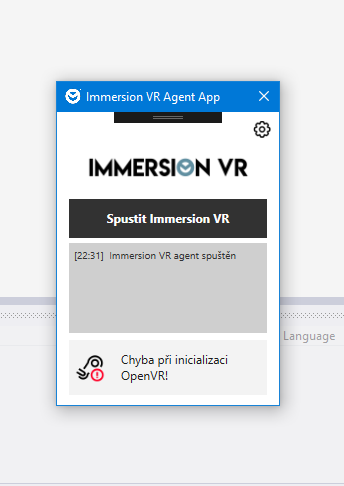
\includegraphics[height=8cm]{src/assets/agent-screen.png}
\caption{Snímek programu agenta}
\end{figure}

Agent je psán také v~jazyce \emph{C\#}. Poskytuje jednoduché uživatelské
rozhraní určené pro obsluhu, které je psáno pomocí knihovny WPF.
Uživatelské rozhraní nabízí tlačítko určené ke spuštění a zastavení celé
aplikace (pokud bude zastavena, přestane se tak i automaticky zapínat
spouštěč) a přehlednou informaci o~aktuálním stavu agenta a úspěšnosti
připojení k~OpenVR systému.

\section{Implementace}\label{implementace}

V~kapitole jsou uvedeny některé konkrétnější detaily implementační fáze
práce. Je popsána struktura celé scény, jakým způsobem jsou ukládána
data o~scénáři výuky, jak je generováno uživatelské rozhraní spouštěče a
jakým způsobem se vytvářel voice-over výuky.

Není tam však ze zřejmých důvodů popsán kompletní postup
implementace. Nezbytnou součástí, která stojí alespoň za zmínku, je
tvorba vizuálu a 3D modelů prostředí, ve kterém se výuka odehrává.

\subsection{Struktura scény}\label{struktura-scuxe9ny}

Herní engine Unity podporuje strukturizaci aplikace do scén. Scény mohou
obsahovat herní objekty (třída \texttt{GameObject}) na které jsou
,,zavěšeny'' komponenty. \autocite{unityscenes} Může jít o~komponenty pracující s~herním
světem, fyzikálními vlastnostmi objektů a nebo o~nejobecnější a
nejmocnější komponentu -- komponentu skriptu. Ta umožňuje k~objektu
připojit vlastní skript v~jazyce C\#, JavaScript či Boo, a naprogramovat
tak logiku daného herního objektu.

Aplikace je strukturována pouze do jedné scény. Ač by na první pohled
dávalo smysl oddělit výuku a spouštěč do samostatných scén, je nutné
brát v~potaz, že přechod z~jedné scény na druhou provází kratší či delší
načítání a implicitně jsou nahrazeny všechny objekty staré scény za
objekty nové scény. I~přesto, že toto chování se dá do určité míry
změnit, je stále nežádoucí, aby v~přechodu mezi výukou a spouštěčem
byla prodleva. Je tak jednodušší obě části spojit do jedné scény a
důkladněji pak strukturovat jednu hlavní scénu.

Herní objekty v~enginu Unity disponují velmi důležitou a užitečnou
funkcí -- mohou být do sebe zanořovány a může jít o~prázdné objekty
pouze s~komponentou \texttt{Transform}, která se stará o~pozicování
v~herním světě. Objekty tak lze sestavovat z~jiných objektů, nebo je
používat pro seskupování objektů.

\newpage

\begin{figure}[h!]
\centering
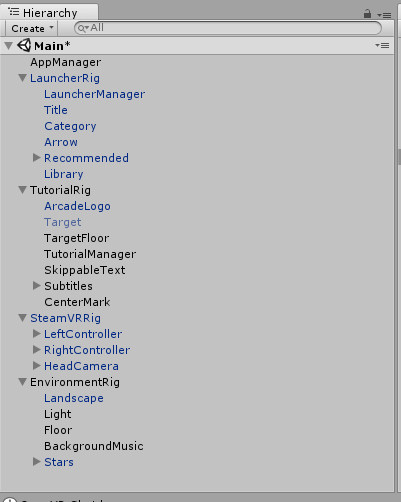
\includegraphics[height=10cm]{src/assets/structure.png}
\caption{Struktura scény}
\end{figure}

Ve scéně aplikace hrají velkou roli dva druhy objektů: tzv.
\textbf{Rigs} (skupiny objektů) a \textbf{Managers} (manažeři). Rigs
slouží k~seskupení objektů se společným účelem. Managers jsou 
objekty se skripty, které řídí určitou část aplikace.

\paragraph{TutorialRig}\label{tutorialrig}

Jedná se o~skupinu všech objektů určených pro výuku. Nachází se zde
\texttt{TutorialManager} (manažer výukové logiky), objekt zobrazující textový přepis scénáře a
další pomocné objekty výuky, jako je objekt s~modelem terče, či objekt
s~modelem loga herny.

\paragraph{LauncherRig}\label{launcherrig}

Obdobně jako \texttt{TutorialRig}, je tento určen k~seskupení všech
objektů spouštěče. Patří sem \texttt{LauncherManager} (manažer logiky spouštěče), prvky
uživatelského rozhraní a objekt knihovny, který má na starosti
vykreslení mřížky dostupných aplikací.

\paragraph{SteamVRRig}\label{steamvrrig}

\texttt{SteamVRRig} je předpřipravenou součástí Steam VR Pluginu pro
\emph{Unity}. Obsahuje objekty reprezentující oba ovladače a headset.
Steam VR Plugin pak zařídí synchronizaci těchto objektů se snímáním
systému virtuální reality. Tyto objekty jsou aktualizovány o~svou
přesnou polohu a rotaci ve fyzickém světě a díky tomu jsou velmi přesně
promítány do herního světa a lze s~nimi tak velmi jednoduše pracovat.

\paragraph{EnvironmentRig}\label{environmentrig}

Seskupení všech objektů prostředí, vizuálních efektů a
statických zvuků. Patří sem objekt vykreslující hory na pozadí,
částicový efekt hvězd na obloze či objekt obstarávající přehrávání hudby
na pozadí.

\subsection{Formát ukládání dat
scénáře}\label{formuxe1t-ukluxe1duxe1nuxed-dat-scuxe9nuxe1ux159e}

Aby se předešlo do kódu napevno zadrátovaného průběhu scénáře, bude
načítán z~externího souboru, který scénář bude popisovat. Díky tomu bude
možné kdykoliv jednoduše provádět úpravy, nebo texty přeložit do
libovolného jazyka. Aplikace díky tomu bude lokalizovatelná.

Interně je formát souboru pojmenován \textbf{STXT} a bude mu příslušet
běžně známá koncovka \texttt{.txt}, jelikož jde o~čitelný textový
soubor, který může být upravován v~běžných editorech.

V~aplikaci se nachází třída \texttt{StxtReader}, jejíž jediný úkol bude
právě čtení tohoto formátu. S~touto třídou souvisí i třída 
\texttt{ScenarioCue}, která je primárně koncipovaná jako datová
struktura, zahrnující všechny údaje o~jednom úseku scénáře.
\texttt{StxtReader} pak principiálně vrací po načtění souboru pole objektů třídy
\texttt{ScenarioCue}. Toto pole je chronologicky seřazeno a celý scénář
bude přehráván postupně podle řazení prvků v~poli.

Vlastnosti třídy \texttt{ScenarioCue} jsou následující:

\begin{itemize}
\tightlist
\item
  časové odsazení od předchozího úseku (offset)
\item
  délka časového úseku (duration)
\item
  identifikátor souvisejícího zvukového úseku (audio cue id)
\item
  text úseku (text)
\item
  činnost úseku (action)
\item
  skupina úseku (groupname)
\end{itemize}

Časové vlastnosti jsou určeny pro pozicování a časování úseků.
Identifikátor zvukového úseku určuje, která zvuková část mluveného textu má být ve
chvíli průchodu úsekem přehrávána. Text úseku je přepisem toho, co
lze ve zvukovém úseku slyšet. Skupina úseku je čistě organizační
záležitostí pro přehlednost \emph{STXT} souboru.

K~popsanému účelu mohlo být využito existujícího formátu \emph{SubRip} \autocite{subrip},
jehož soubory mají koncovku \texttt{.srt} a jsou hojně využívány pro
tvorbu titulků k~filmům a seriálům. \emph{SubRip} však pracuje
s~neúměrnou časovou značkou k~účelu aplikace a nepodporuje jiné vlastnosti
časových úseků, pouze jejich text.

\subsubsection{Syntaxe STXT souboru}\label{syntaxe-stxt-souboru}

U~syntaxe formátu byl kladen důraz na jednoduchost implementace čtení
formátu. Obecně lze syntaxi definovat následovně:

\begin{minted}[bgcolor=codebg]{text}
#<groupname>
<offset>;<duration>;<audio cue id>:(<text>|%<action>)
[<offset>;<duration>;<audio cue id>:(<text>|%<action>)] ...

[#<groupname>
<offset>;<duration>;<audio cue id>:(<text>|%<action>)
[<offset>;<duration>;<audio cue id>:(<text>|%<action>)]] ...

...
\end{minted}

Kde bloky označené \texttt{\textless{}} a \texttt{\textgreater{}} jsou
bloky hodnot, bloky označené \texttt{{[}} a \texttt{{]}} jsou nepovinné
bloky a bloky ve tvaru \texttt{(\ A\ \textbar{}\ B\ )} představují
možnost alternativy (A~nebo B). Skupiny bloků, které jsou odděleny řádky
lze libovolně opakovat. Minimální počet takových bloků je 1. Skupiny
není nutné oddělovat prázdnými řádky. Podporuje to však čitelnost souboru.

\newpage

Významy bloků jsou uvedeny v~tabulce:


\extrarowsep=4pt\begin{longtabu}{XX}
\toprule
Název bloku & Funkce bloku\tabularnewline
\midrule
\endhead
\texttt{\textless{}groupname\textgreater{}} & Název
skupiny\tabularnewline
\texttt{\textless{}offset\textgreater{}} & Časové odsazení od
předchozího úseku v~sekundách\tabularnewline
\texttt{\textless{}duration\textgreater{}} & Doba trvání daného časového
úseku v~sekundách\tabularnewline
\texttt{\textless{}audio\ cue\ id\textgreater{}} & Identifikátor
zvukového úseku\tabularnewline
\texttt{\textless{}text\textgreater{}} & Text úseku (přepis zvukového
úseku)\tabularnewline
\texttt{\textless{}action\textgreater{}} & Činnost, která se má v~úseku
provést\tabularnewline
\bottomrule
\end{longtabu}

Pro lepší představu je níže uveden krátký úryvek \emph{STXT} souboru
z~aplikace, na kterém lze snadněji vidět jeho praktické použití.

\begin{minted}[bgcolor=codebg]{text}
#intro
1;0;0:%showlogo
2;2.4;0:Vítejte v~herně Virtualnirealita.cz!
0;3.6;0:Tato krátká výuka vás provede vstupem do virtuální reality.
0;0;0:%hidelogo

#skippable
0;0;1:%showskiptxt
0;6.5;1:Pokud s~virtuální realitou již máte zkušenosti...
0;0;1:%hideskiptxt

...
\end{minted}

\newpage

Činnosti jsou, na rozdíl od textů a časování, pevně určené, protože jsou
daleko komplexnější a mnohem méně parametrizovatelné. Pro referenci je
tak uvedena kompletní tabulka všech použitelných činností.

\begin{longtabu} to \textwidth {XX}
\toprule

Název činnosti
& 
Popis činnosti
\tabularnewline
\midrule
\endhead
\texttt{\%showlogo}
& 
Zobrazí před uživatelem logo herny.
\tabularnewline

\texttt{\%hidelogo}
& 
Skryje logo herny.
\tabularnewline

\texttt{\%showskiptxt}
& 
Zobrazí informaci o~možnosti přeskočit výuku.
\tabularnewline

\texttt{\%hideskiptxt}
& 
Skryje informaci o~možnosti přeskočit výuku.
\tabularnewline

\texttt{\%waitforuserraise}
& 
Pozastaví se a čeká, dokud uživatel nezvedne ruce před sebe.
\tabularnewline

\texttt{\%highlighttrigger}
& 
Zvýrazní na ovladači tlačítko spouště.
\tabularnewline

\texttt{\%givelaser}
& 
Přidá uživateli možnost používat laserové ukazovátko.
\tabularnewline

\texttt{\%waitforusertargethit}
& 
Pozastaví se a čeká, dokud uživatel netrefí laserovým paprskem
terč.
\tabularnewline

\texttt{\%highlightside}
& 
Zvýrazní boční tlačítko na ovladači.
\tabularnewline

\texttt{\%waitforside}
& 
Pozastaví se a čeká, dokud uživatel nestiskne boční tlačítko.
\tabularnewline

\texttt{\%highlighttouchpad}
& 
Zvýrazní na ovladači dotykovou plochu.
\tabularnewline

\texttt{\%waitforusercolor}
& 
Pozastaví se a čeká, dokud uživatel nezvolí na ovladači barvu.
\tabularnewline

\texttt{\%highlightmenu}
& 
Zvýrazní menu tlačítko na ovladači.
\tabularnewline

\texttt{\%highlightsystem}
& 
Zvýrazní systémové tlačítko na ovladači.
\tabularnewline

\texttt{\%gotolibrary}
& 
Zobrazí spouštěč.
\tabularnewline

\texttt{\%skip}
& 
Přeskočí výuku.
\tabularnewline
\bottomrule
\end{longtabu}

Stále je ale pružnost výuky do určité míry zachována a je dostatečně
přizpůsobitelná. Tyto akce lze přeskládat jinak, spouštět v~jiné časy,
případně je i vynechat.

\subsection{Mluvený text průvodce
výuky}\label{mluvenuxfd-text-prux16fvodce-vuxfduky}

Dokončená implementace postupování výuky a zobrazení přepisu si žádala
přidání mluveného textu do aplikace. Součástí práce bylo nadabování
mluvy, jeho post-produkce a import do projektu.

Při dabování byl dbán důraz na rychlost mluvy, aby výuka nebyla
zdlouhavá, ale zároveň byla kontrolována srozumitelnost projevu a pauzy
na vhodných místech.

Výsledná délka pouze mluveného textu je 116 vteřin. Práce se zvukovými
soubory dělá výslednou délku výuky odlišnou od délky samotného mluveného
textu. Mezi jednotlivé části jsou vloženy mezery, nebo některé části
mohou být uživatelem přeskočeny. 

Délka výuky s~vloženými mezerami a bez
čekání na vstup uživatele je 124 vteřin. Právě vstup uživatele dělá tuto
hodnotu velmi kolísavou. Předběžným odhadem bude výuka \textbf{100s až
160s} dlouhá. Reálné délky výuky však odhalí až testování.

\begin{figure}[h!]
\centering
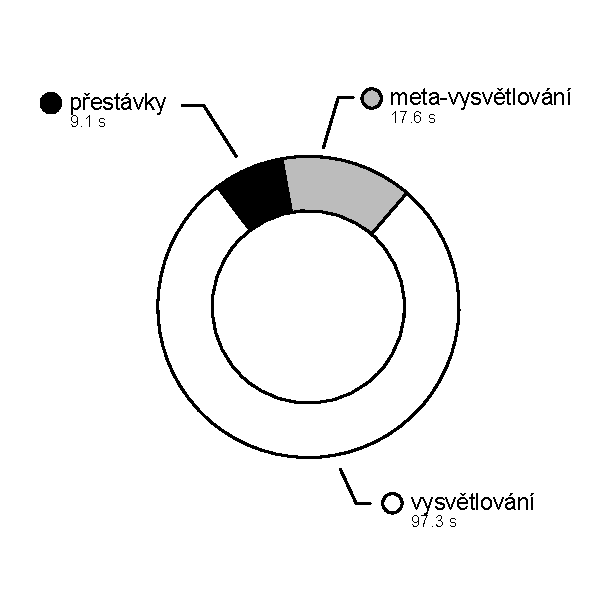
\includegraphics[height=9cm]{src/assets/time-chart.pdf}
\caption{Rozdělení času mluveného textu}
\end{figure}

Z~pozdní analýzy subjektivně plyne, že jsou užitečné a neužitečné
části mluvy rozděleny správně. Přibližně tři čtvrtiny jsou věnovány
tomu nejdůležitějšímu -- vysvětlování, a jedna čtvrtina je zaplněna
meta-vysvětlováním a pauzami, kde pauzy konkrétně zaujímají pouze přes 7
\% celého času.

Lze tak tvrdit, že výuka je efektivní a splní požadavek \emph{N-04} na
časovou efektivitu.

\section{Nedostatky}\label{nedostatky}

Omezený čas na tvorbu aplikace ovlivnil výsledek a tak nebyla splněna realizace
některých funkí, které byly navrženy.

Kategorizace byla implementována pouze částečně. Implementoval se funkční
prvek rozhraní, ale vnitřně nebylo implementováno seskupování her do kategorií.

Také nebylo implementováno žádné prostředí, ve kterém by mohla obsluha herny
vybírat oblíbené hry, specifikovat, zda se má zobrazovat celá knihovna her
a další proměnné. Všechna tato konfigurace je zapsána
v~uživatelsky nepřívětivém souboru konfigurace.
